\section{Results}\label{results}

\boldif{Results from interviews indicated that a common model of operating with merge conflicts exists.}
To understand how developers manage merge conflicts, we asked interview participants to describe their current processes for handling merge conflict.

\boldif{\textit{Add anecdotal quotes and descriptions from interviews to highlight these observations.}}
Participants talked about different steps that they follow, including using tools that alert them to potential or current merge conflicts, processes for analyzing and understanding conflicting code prior to implementing a resolution, and the use of tools for validating that their resolution worked.
As an example, P3 said:
\begin{quoting}
\textit{``Part of my job on the integration team requires that I check for bad regressions. I use scripts to track patches as they're being backported, so I know when and where to look if [a patch] introduces a conflict. [\ldots] And once I've fixed [the conflict], I try to compare with the previous version to make sure [the code] works in a similar way.''}
\end{quoting}

\boldif{Provide descriptions that link the stages of Merge Conflict model to this quote. Use it to drive description of simplified model description paragraph}

\boldif{Based on these anecdotal observations, we construct an initial model of the processes that developers employ when working with merge conflicts, see Fig.~\ref{model}.}
Our interview and survey results suggest that developers follow a series of phases through which they manage the life-cycle of individual merge conflicts.
We construct a model of the developer processes for managing merge conflicts and examine each phase in detail.
Figure~\ref{model} provides an illustration of this model. 
It consists of four phases: \emph{awareness, planning, resolution,} and \emph{evaluation.}

\boldif{Discuss the fact that no other studies have shown that a model exists for merge conflicts}

\begin{figure}[!htbp]
\centering
\fbox{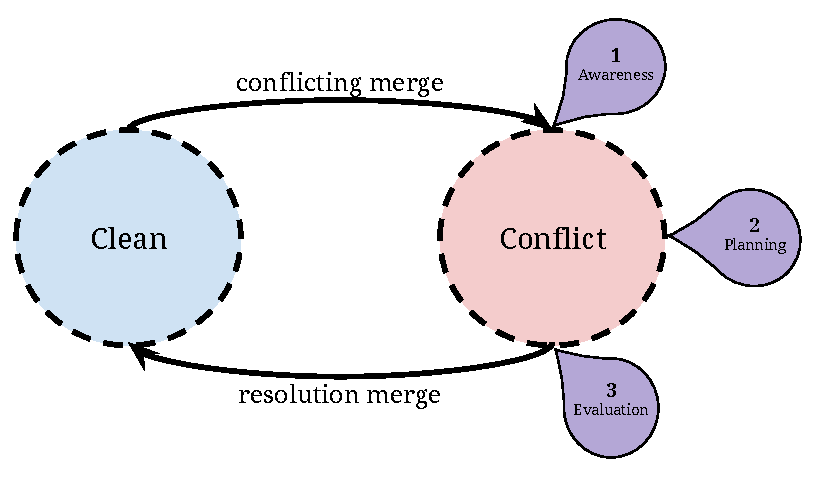
\includegraphics[width=0.90\textwidth,keepaspectratio]{imgs/MergeConflictModel}}
\caption{Model of Developer Processes for Managing Merge Conflicts. Developers alternate between \textit{clean} and \textit{conflicting} states of code. Beginning from (1)~\textit{development}, developers maintain (2)~\textit{awareness} of conflicts within the codebase in different ways. Once aware, developers begin (3)~\textit{planning} for a (4)~\textit{resolution} to fix the conflict. And finally, developers (5)~\textit{evaluate} the effectiveness of their deployed resolutions (returning to \emph{planning} if the resolution failed).\vspace*{-0.3\baselineskip}}
\label{model}
\end{figure}

\boldif{Awareness is how developers become aware}
First, the \emph{awareness} phase consists of the actions developers take to become aware of merge conflicts.
This could be passive, as the developer will become aware of a merge conflict when attempting to merge changes or perform a pull.
At the other end of the spectrum are developers who \emph{proactively} monitor for merge conflicts as they write code.
They are actively looking for changes that might be problematic, either manually or through the use of specialized tools.

\boldif{Planning is when developers plan their future actions}
Second, the \emph{planning} phase occurs after the developer has become aware that a conflict has occurred, and they are about to tackle the conflict.
This includes the decision of when they will try and resolve the conflict.
Some developers might try and resolve it immediately, while others might postpone the resolution.
Some might change their strategy depending on the conflict, incoming deadlines, or availability of resources.
This also includes other actions, such as if they are going to tackle the conflict alone, or collaborate with other developers knowledgeable in the area of conflict~\cite{CostaSarma}.

\boldif{Resolution is the action of implementing a resolution. Mundane and well understood, so we focus on the other three.}
Third, the \emph{resolution} phase represents the implementation of the planned resolution.
Several tools exist that help in this phase~\cite{nishimura,mens2002state,Brun2011}.
Here we focus on the difficulties that developers face during these resolution implementations (see Section~\ref{RQ2}).

\boldif{Evaluation is how developers check that their solution is correct}
Finally, after the conflict has been resolved, developers enter in the \emph{evaluation} phase.
In this phase, the developer has to evaluate their resolution before considering the conflict as resolved.
This is to ensure the correctness of the resulting code.
Possible actions during this stage includes compiling the source code.
Developers wanting more guarantees can go a step further and run the tests.
Finally, some groups have policies such as code reviews that need to be performed on the merge conflict resolution.
 
\boldif{To explore and validate this model, we asked developers to reflect upon how they become aware of merge conflicts, how they plan for merge conflict resolutions, and how they evaluate their resolutions in the \textit{Processes Survey}.}
In order to explore and validate this model, and our assumptions, we conducted the \emph{Processes Survey}.
Our aim in this survey was to understand how developers become aware of merge conflicts (what steps they take, what tools they use, etc.).
Also, we wanted to investigate their strategies for dealing with merge conflicts and how they decide whether the resolution has addressed all of their concerns.

Results are categorized according to the life-cycle of merge conflicts; with specific results for the \textit{awareness} (Section~\ref{RQ1}), \textit{planning} (Section~\ref{RQ2}), and \textit{evaluation} phases (Section~\ref{RQ3}).
We then present the difficulties that developers experience when managing merge conflicts (Section~\ref{RQ4}).
And finally, we examine the gaps in tool support for managing merge conflicts according to developer's needs (Section~\ref{RQ5}).

%!TEX root = main.tex

\subsection{\textbf{RQ1:} Ho do software developers manage merge conflicts?}\label{RQ1}

\boldif{Results from interviews indicated that a common model of operating with merge conflicts exists.}
To understand how developers manage merge conflicts, we asked interview participants to describe their current processes for handling merge conflict.

\boldif{\textit{Add anecdotal quotes and descriptions from interviews to highlight these observations.}}
Participants talked about different steps that they follow, including using tools that alert them to potential or current merge conflicts, processes for analyzing and understanding conflicting code prior to implementing a resolution, and the use of tools for validating that their resolution worked.
As an example, P3 said:
\begin{quoting}
\textit{``Part of my job on the integration team requires that I check for bad regressions. I use scripts to track patches as they're being backported, so I know when and where to look if [a patch] introduces a conflict. [\ldots] And once I've fixed [the conflict], I try to compare with the previous version to make sure [the code] works in a similar way.''}
\end{quoting}

\boldif{Provide descriptions that link the stages of Merge Conflict model to this quote. Use it to drive description of simplified model description paragraph}

\boldif{Based on these anecdotal observations, we construct an initial model of the processes that developers employ when working with merge conflicts, see Fig.~\ref{model}.}
Our interview and survey results suggest that developers follow a series of phases through which they manage the life-cycle of individual merge conflicts.
We construct a model of the developer processes for managing merge conflicts and examine each phase in detail.
Figure~\ref{model} provides an illustration of this model. 
It consists of four phases: \emph{awareness, planning, resolution,} and \emph{evaluation.}

\boldif{Discuss the fact that no other studies have shown that a model exists for merge conflicts}

\begin{figure}[!htbp]
\centering
\fbox{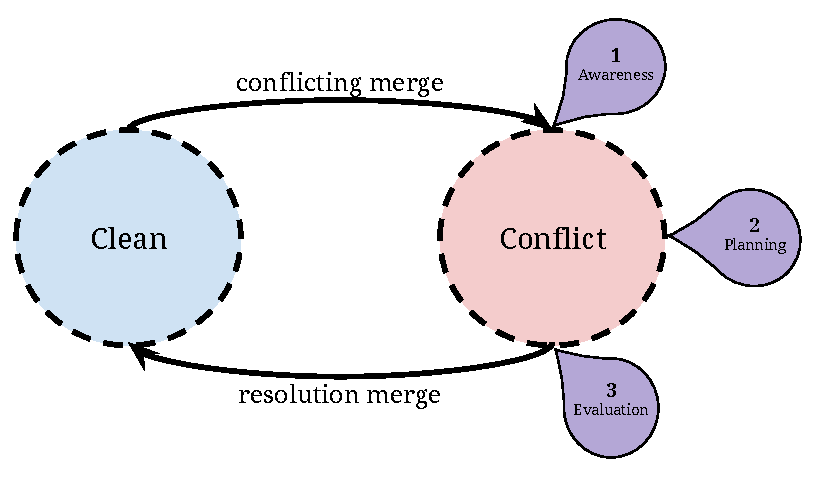
\includegraphics[width=0.90\textwidth,keepaspectratio]{imgs/MergeConflictModel}}
\caption{Model of Developer Processes for Managing Merge Conflicts. Developers alternate between \textit{clean} and \textit{conflicting} states of code. Beginning from (1)~\textit{development}, developers maintain (2)~\textit{awareness} of conflicts within the codebase in different ways. Once aware, developers begin (3)~\textit{planning} for a (4)~\textit{resolution} to fix the conflict. And finally, developers (5)~\textit{evaluate} the effectiveness of their deployed resolutions (returning to \emph{planning} if the resolution failed).\vspace*{-0.3\baselineskip}}
\label{model}
\end{figure}

\boldif{Awareness is how developers become aware}
First, the \emph{awareness} phase consists of the actions developers take to become aware of merge conflicts.
This could be passive, as the developer will become aware of a merge conflict when attempting to merge changes or perform a pull.
At the other end of the spectrum are developers who \emph{proactively} monitor for merge conflicts as they write code.
They are actively looking for changes that might be problematic, either manually or through the use of specialized tools.

\boldif{Planning is when developers plan their future actions}
Second, the \emph{planning} phase occurs after the developer has become aware that a conflict has occurred, and they are about to tackle the conflict.
This includes the decision of when they will try and resolve the conflict.
Some developers might try and resolve it immediately, while others might postpone the resolution.
Some might change their strategy depending on the conflict, incoming deadlines, or availability of resources.
This also includes other actions, such as if they are going to tackle the conflict alone, or collaborate with other developers knowledgeable in the area of conflict~\cite{CostaSarma}.

\boldif{Resolution is the action of implementing a resolution. Mundane and well understood, so we focus on the other three.}
Third, the \emph{resolution} phase represents the implementation of the planned resolution.
Several tools exist that help in this phase~\cite{nishimura,mens2002state,Brun2011}.
Here we focus on the difficulties that developers face during these resolution implementations (see Section~\ref{RQ2}).

\boldif{Evaluation is how developers check that their solution is correct}
Finally, after the conflict has been resolved, developers enter in the \emph{evaluation} phase.
In this phase, the developer has to evaluate their resolution before considering the conflict as resolved.
This is to ensure the correctness of the resulting code.
Possible actions during this stage includes compiling the source code.
Developers wanting more guarantees can go a step further and run the tests.
Finally, some groups have policies such as code reviews that need to be performed on the merge conflict resolution.
 
\boldif{To explore and validate this model, we asked developers to reflect upon how they become aware of merge conflicts, how they plan for merge conflict resolutions, and how they evaluate their resolutions in the \textit{Processes Survey}~(S1).}
In order to explore and validate this model, and our assumptions, we conducted the \emph{Processes Survey}~(S1).
Our aim in this survey was to understand how developers become aware of merge conflicts (what steps they take, what tools they use, etc.).
Also, we wanted to investigate their strategies for dealing with merge conflicts and how they decide whether the resolution has addressed all of their concerns.

\boldif{We present the results to these research questions in Sections~\ref{RQ1a}, \ref{RQ1b}, and \ref{RQ1c}.}
Sections~\ref{RQ1a}, \ref{RQ1b}, and \ref{RQ1c} presents the results to these research questions.

\subsubsection{\textbf{RQ1a:} How do software developers become \textbf{aware} of merge conflicts?}\label{RQ1a}

\boldif{Developers use 2 methods for becoming aware of merge conflicts: proactive and reactive.}
From the \textit{Processes Survey}~(S1) we found that 29.41\% of participants do not actively monitor for merge conflicts during their development activities.
For the rest of the developers who answered with \emph{yes} or \emph{sometimes} (61.77\%), we identified 61 different tools mentioned in 126 instances.

\nsubsection{Reactive and Proactive Monitoring for Merge Conflicts}

\boldif{Reactive detection only notifies developers that a merge conflict \emph{has happened}. Developers use it to minimize the size/complexity of the conflict, or it's impact on the team.}
Reactive monitoring for merge conflicts notifies the developer that a conflict has already occurred.
However, developers still use this process to manage or reduce the complexity of a conflict.
For the developers who answered that they monitor for merge conflicts (replied either \emph{yes} or \emph{sometimes}), we found that 73.68\% (42 out of 57 responses; 6 participants left this field blank) described reactive processes.
For example, participant S1--48 said they use integration tools to detect merge problems before they advance to testing:
\begin{quotation}
	[\ldots] integration tests tell us if builds are breaking and we use those to locate merge conflicts. [\ldots] we use it to catch merge bugs before they go to smoke testing for release
\end{quotation}
And participant S1--64 mentioned that they try to solve merge conflicts early in order to minimize disruptions to the team:
\begin{quotation}
	We try to catch conflicts early so that fewer developers have to be involved in looking at broken code.
\end{quotation}

\boldif{Proactive monitoring allows devs to detect MC before they happen. However, it is more involved, as it requires a lot more manual effort from the developers.}
Proactive monitoring allows developers to preemptively catch merge conflicts before they happen.
15 participants (14.71\%) mentioned they achieved this by manually tracking incoming changes, such as participant S1--35 who indicated:
\begin{quotation}
	I monitor commit logs before I begin merging branches so that I see any potentially overlapping code that will break the merge.
\end{quotation}
Other teams rely more on communication.
This can happen during regular team meetings, to make sure that everybody is aware of each other's tasks, for example participant S1--46 said:
\begin{quotation}
	[\ldots] standups allow us to know where everyone is working that week.
\end{quotation}
While 10 participants (9.80\%) indicated that they broadcast their changes in order to notify team members if they will make breaking changes.
For example, participant S1--102 indicated that team members:
\begin{quotation}
	[\ldots] send emails before making breaking changes to the API or related sub-modules.
\end{quotation}

\boldif{Developers do not regularly actively monitor for merge conflicts. ...}
To conclude, only a third of developers actively monitor for merge conflicts.
When developers are caught unaware of the conflict, they are more likely to be interrupted by it.
This can lead to more frustration, as they do not have any warning of when the conflict will occur and whether they have the time to deal with it immediately.

\nsubsection{Tools for Monitoring for Merge Conflicts}

\boldif{The tools that developers use allow for only a \emph{reactive} approach.}
Examining the tools used by participants with reactive processes, we find that 87.72\% of these participants rely on version control systems (e.g. Git, SVN, TFS, CVS), while 21.05\% use continuous integration systems (e.g. Jenkins, Travis CI, TeamCity).
Table~\ref{s1_toolset} presents the top 10 tools developers use when monitoring for merge conflicts, including the totals for both reactive and proactive strategies.

Additionally, we examine the tools used by participants with proactive processes.
We find that all participants with a proactive strategy rely on version control systems, and 33.33\% use continuous integration systems.
Additionally, 26.66\% of proactive participants use code analysis tools (e.g. SonarQube, Code Climate).

We find that the majority of tools used by developers for merge conflict monitoring are built to only support reactive strategies, and that multiple tools must be used in conjunction for a proactive approach.

%\boldif{Devs do not use existing workspace awareness tools that come from the acadmemia.}
%When collaborating, developers generally rely on passive communication tools, like email, to coordinate.
%Developers are currently not leveraging the functionalities provided by many research prototypes (e.g., Palant\'{i}r~\cite{palantir}, Crystal~\cite{Brun2011}) that are specifically designed to facilitate proactive conflict detection.

\begin{table}[!htbp]
\renewcommand{\arraystretch}{1.3}
\caption{Merge Awareness Toolsets (Top 10) from Processes Survey (S1)}
\label{s1_toolset}
\centering
\begin{tabularx}{\textwidth}{ll|cc|c}
\toprule
% \textbf{Par.}\parnote{Par. = Total number of survey participants using each tool.}
% \vspace*{-0.3\baselineskip}
  \parnoteclear % tabularx will otherwise add each note thrice
  Tool\parnote{\textit{Processes Survey}~(S1) participants were allowed to provide multiple tools. 57 out of 102 participants (56\%) indicated the use of at least one merge awareness tool.} & Description & Proactive\parnote{Participants using this tool with a proactive strategy.} & Reactive\parnote{Participants using this tool with reactive strategy.} & Total\parnote{Total number of survey participants using each particular tool.}\\
\midrule
  Git & Version Control System & 10 & 30 & 40\\
  Email (unspecified) & Email Client or System & 2 & 4 & 6\\
  GitHub & Project Hosting Site & 2 & 5 & 7\\
  SVN & Version Control System & 0 & 4 & 4\\
  Visual Studio & IDE & 1 & 2 & 3\\
  PagerDuty & IT Incident Manag. Sys. & 0 & 3 & 3\\
  GitLab & Project Hosting Site & 2 & 1 & 3\\
  Jenkins & Continuous Integration & 0 & 3 & 3\\
  VCS (unspecified) & Version Control System & 2 & 2 & 4\\
  Team Foundation Server & Version Control System & 1 & 1 & 2\\
\bottomrule
\end{tabularx}
\parnotes
\end{table}


\boldif{Therefore their approaches are mostly \emph{reactive,} and their tool selection reflects that.}
To summarize, we find that developers employ \emph{reactive} processes, even if they are proactive in monitoring for merge conflicts once they have occurred.
This can be seen as a consequence of the tools that developers have at their disposal.
All the tools mentioned support only a \emph{reactive} approach, which biases developers towards one particular solution.
If developers want a more \emph{proactive} approach, then based on the tools they use, they need to come up with their own solution.
The most often cited techniques involve increasing communication among developers.
While this technique might be effective in small teams, it scales very poorly and cannot be effectively used in larger organizations~\cite{brooks1974mythical}.

\boldif{All the above point towards a need for better collaborative tools, that promote a proactive approach}
Finally, our results point to the conclusion that developers are not aware of existing proactive tools (e.g. Palant\'{i}r~\cite{sarma_palantir:_2003}, Crystal~\cite{Brun2011}), and are therefore not leveraging those tools to actively monitor for merge conflicts.
However, developers are trying to mitigate the severity of merge conflicts by attempting to resolve them as soon as they become aware.

\subsubsection{\textbf{RQ1b:} How do software developers \textbf{plan} for merge conflict resolutions?}\label{RQ1b}

\boldif{Developers use different strategies for dealing with MC}
When encountering a merge conflict, developers follow different strategies.
They can either: (a) defer the merge conflict to a later date, or; (b) solve the conflict.
In the \textit{Processes Survey}~(S1) we sought an understanding of these strategies and when developers use them.
The tools that developers use when implementing merge conflict resolutions are discussed in Section~\ref{RQ3}.

\nsubsection{Deferring Responses to Merge Conflicts}

\boldif{25\% of developers consider all conflicts as being equally urgent.}
One quarter of our participants consider all merge conflicts to be equally urgent.
This means that they will always solve the conflict as soon as the 
We can assume that most developers will interrupt their work regardless of the type of merge conflict.
Therefore, they will give the same level of attention, for example, to a conflict generated by whitespace or formatting changes, as a conflict that is generated by overlapping logical changes. 
%TODO: Make sure this fits in the flow.

\boldif{The first option is that they might defer the MC, for a later time}
The easiest option when encountering a merge conflict is to simply not deal with it.
Indeed, we found that 56.18\% of participants have deferred at least once when responding to a merge conflict.
The reasons for deferring are varied and listed in Table~\ref{s1_deferring_response}.

The location and complexity of conflicting code (D1, D2) were the most selected factors, and match the top difficulty factors of merge conflicts (F1, F2) as described in Section~\ref{difficulty-factors}.
% TODO Add a conclusion statement about the meaning of these factors being top in both tables.

As the third most selected factor, \textit{ownership of the conflicting code}~(D3) indicates that the deferral is not always temporal, but can also be logistical when developers defer to other team members.
Participant S1--8 succinctly defines the role ownership impacts his workflow as:
\begin{quotation}
	Code is mine? I fix it. Code is others? I submit PR or bug reports.
\end{quotation}
We additionally asked participants to rate the degree to which code ownership factors into their overall merge conflict strategy, and participants indicate that code ownership factors \textit{about half the time} in their strategy of code ownership (mean: $3.21$ on a 5-point Likert-type scale).
Only 10.11\% of participants indicated that code ownership \textit{never} factors into their resolution strategy.

\begin{table}[!htbp]
\renewcommand{\arraystretch}{1.2}
\caption{Factors in Deferring Responses to Merge Conflicts from Processes Survey (S1)}
\label{s1_deferring_response}
\centering
\begin{tabularx}{\textwidth}{>{\rowmac}c | >{\rowmac}l | >{\rowmac}c | >{\rowmac}r <{\clearrow}}
\toprule
  \parnoteclear % tabularx will otherwise add each note thrice
  Factor & Description & \# Selections\parnote{\textit{Processes Survey}~(S1) participants were allowed to select multiple factors. 44 out of 102 participants (43\%) selected more than one factor.\vspace*{-0.9\baselineskip}} & Percentage (\%)\textsuperscript{i} \\
\midrule
  D1 & Complexity of the conflicting code & 36 & 25.00\% \\
  D2 & Number of conflicting code locations & 32 & 22.22\% \\
  D3 & Ownership of the conflicting code & 25 & 17.36\% \\
  D4 & Size of the conflicting code & 20 & 13.89\% \\
  D5 & Approaching deadlines & 13 & 9.03\% \\
  D6 & Work schedule constraints & 2 & 1.39\% \\
  D7 & Other\hspace{4.6cm} & 7 & 4.86\% \\
\bottomrule
\end{tabularx}
\parnotes
\end{table}

\boldif{60\% of developers defer a merge conflict, at least once. However, there doesn't seem to be a systematic understanding of the effect of such a deferral.}
%Our study results indicate that 60\% of developers have deferred a merge conflict at least once. 
While developers have listed multiple reasons for deferral, two stand out: complexity and the number of conflicting locations.
Both of these reasons indicate that a developer is more likely to defer if the conflict resolution appears to be lengthy, either because the potential changes are non-trivial or because there are many smaller conflicts requiring the developers' attention.

\nsubsection{Deferring Response to Merge Conflicts}

\boldif{Deferring can have bad consequences, including increased complexity and delaying features. Organizations have sometimes changed the policy to prevent this.}
Deferring the merge conflict resolution comes with a price.
Table~\ref{effects-deferral} shows the top effects of deferring a response to a merge conflict.
The most common effect was that developers have had to stop the development (\emph{Stop the Presses,} 15 responses) in order to resolve the conflicts.
This halt in development includes asking team members to also refrain from adding any additional code into the codebase.
The second most common effect is the \textit{increased complexity} of the conflicts (E2), reported by nine participants.
Participant S1--93 noted that:
\begin{quotation}
	Deferring a merge conflict simply kicks the can down the road (or off a cliff). Typically resolving the conflict only gets more difficult as time passes.
\end{quotation}
Participant S1--70 even hinted that the increased complexity can be quite severe, on an order of magnitude greater than if the conflict were addressed immediately:
\begin{quotation}
	Untangling takes days instead of minutes when it gets too out of hand.
\end{quotation}
In some cases, features had to be removed from releases, in order for integration problems to be mitigated and the conflict to be successfully resolved. S1--5 said:
\begin{quotation}
	We have had several releases come up short in new features because they got delayed by integration problems.
\end{quotation}
Finally, in order to prevent similar problems arising, some organizations have instituted \textit{policy changes} (E4) to prevent this from happening in the future. Participant S1--46 said:
\begin{quotation}
	We've had devs push a bunch of code up before going on holiday and mucking up a release, so we've instituted an all hands on deck policy for the 2 weeks leading up to a major release
\end{quotation}

\boldif{However, some effect can be severe, including impact to customers, or having to reimplement features.}
In one extreme case, participant S1--9 reported that an unresolved merge conflict affected production software (E7), which resulted in downtime of the product, as it broke functionality:
\begin{quotation}
	Broke the app for customers until we could get a patch pushed [\ldots].
\end{quotation}
Finally, the merge conflicts can get too severe and intractable for developers to cope with the complexities.
In these types of situations, developers have to resort to the \emph{Nuclear Option} (E5), where they scrap their changes and manually reimplement them.
Such as in the case of S1--102, who said:
\begin{quotation}
	Uh.... KABOOM! More changes came in and everything piled up. Nothing to do but wipe it all back to clean and start trying to piece things back together.
\end{quotation}

\begin{table}[!htbp]
\renewcommand{\arraystretch}{1.2}
\caption{Effects of Deferring Response to a Merge Conflict from Processes Survey (S1)}
\label{effects-deferral}
\centering
\begin{tabularx}{\textwidth}{>{\rowmac}c | >{\rowmac}l | >{\rowmac}c | >{\rowmac}r <{\clearrow}}
\toprule
  \parnoteclear % tabularx will otherwise add each note thrice
  Effect & Description & \# Participants\parnote{46 out of 102 participants (45.1\%) provided a description of the effects of deferring.\vspace*{-0.8\baselineskip}} & Percentage (\%)\textsuperscript{i} \\
\midrule
  E1 & Stop the Presses & 15 & 32.61\% \\
  E2 & Increased complexity & 9 & 19.57\% \\
  E3 & Non-operation effects & 5 & 10.87\% \\
  E4 & Policy/cultural changes & 3 & 6.52\% \\
  E5 & The Nuclear Option & 2 & 4.35\% \\
  E6 & Physical manifestations & 1 & 2.17\% \\
  E7 & Impact beyond the organization \hspace{1cm} & 2 & 2.17\% \\
\bottomrule
\end{tabularx}
\parnotes
\end{table}
\vspace{0.8em}

\boldif{The results of such a deferral can be disastrous. However, it is difficult to make an assessment of the effect of the deferral when the decision to defer is being made.} 
The results of deferring can be disastrous. 
%Participants reported having to throw away code (the \emph{Nuclear Option}) and even rising to the level of customers and users experiencing broken functionality and loss of access.
However, it is difficult to assess a deferral to determine if it will turn a single merge conflict into a larger problem.
Tools could provide such information; responding to developers with enough information to make accurate and informed decisions in order to prevent further issues down the line.

\nsubsection{Attempting Resolution \& Initial Strategies}

\boldif{If they have not deferred, they need to understand the (changes in the) conflict}
When developers don't defer their response, they have to resolve the conflicts now.
They primarily approach merge conflicts by \textit{examining the merge} (U1), \textit{analyzing or manipulating the code} (U2), or \textit{examining the code} (U3).
Table~\ref{s1_understanding_code} lists all six strategies described by the \textit{Processes Survey}~(S1) participants.

\begin{table}[!htbp]
\renewcommand{\arraystretch}{1.2}
\caption{Initial Strategies for Understanding Conflicting Code from Processes Survey (S1)}
\label{s1_understanding_code}
\centering
\begin{tabularx}{\textwidth}{>{\rowmac}c | >{\rowmac}l | >{\rowmac}c | >{\rowmac}r <{\clearrow}}
\toprule
  \parnoteclear % tabularx will otherwise add each note thrice
  Strategy & Description & \# Participants\parnote{79 out of 102 participants (77\%) provided a description of their initial strategy.\vspace*{-0.3\baselineskip}} & Percentage (\%)\textsuperscript{i} \\
\midrule
  U1 & Examining the merge & 26 & 32.91\% \\
  U2 & Analysis/manipulation of the code & 19 & 24.05\% \\
  U3 & Examining the code & 18 & 22.79\% \\
  U4 & Focus on design concerns & 8 & 10.13\% \\
  U5 & Examine project organization & 6 & 7.60\% \\
  U6 & No strategy\hspace{3.5cm} & 2 & 2.53\% \\
\bottomrule
\end{tabularx}
\parnotes
\end{table}
\vspace{0.8em}

\boldif{The most common strategies for understanding the conflict are examining the conflict and analysis/manipulation of the code.}
Participant S1--44 described their strategy of \textit{examining the merge}~(U1) as:
\begin{quotation}
	Reviewing the most recent commits (comments and code) to see whether it's a shallow conflict or not.
\end{quotation}
	And participant S1--69 indicated their strategy of analyzing the code (U2) involves:
\begin{quotation}
[\ldots] determining if the merge conflict involves important functionality; stepping through with a debugger helps.
\end{quotation}
Overall, we find that developers initially focus on the code involved in the merge conflict or information related to the merge itself.

\boldif{Surprisingly, some developers do not have a strategy for MCR}
Surprisingly, we found that two of our participants (2.53\% of participants) indicated that they \textit{``don't have a strategy''} or \textit{``mostly try to fix it as soon as possible.''}

%\begin{figure}[!htbp]
%\centering
%\fbox{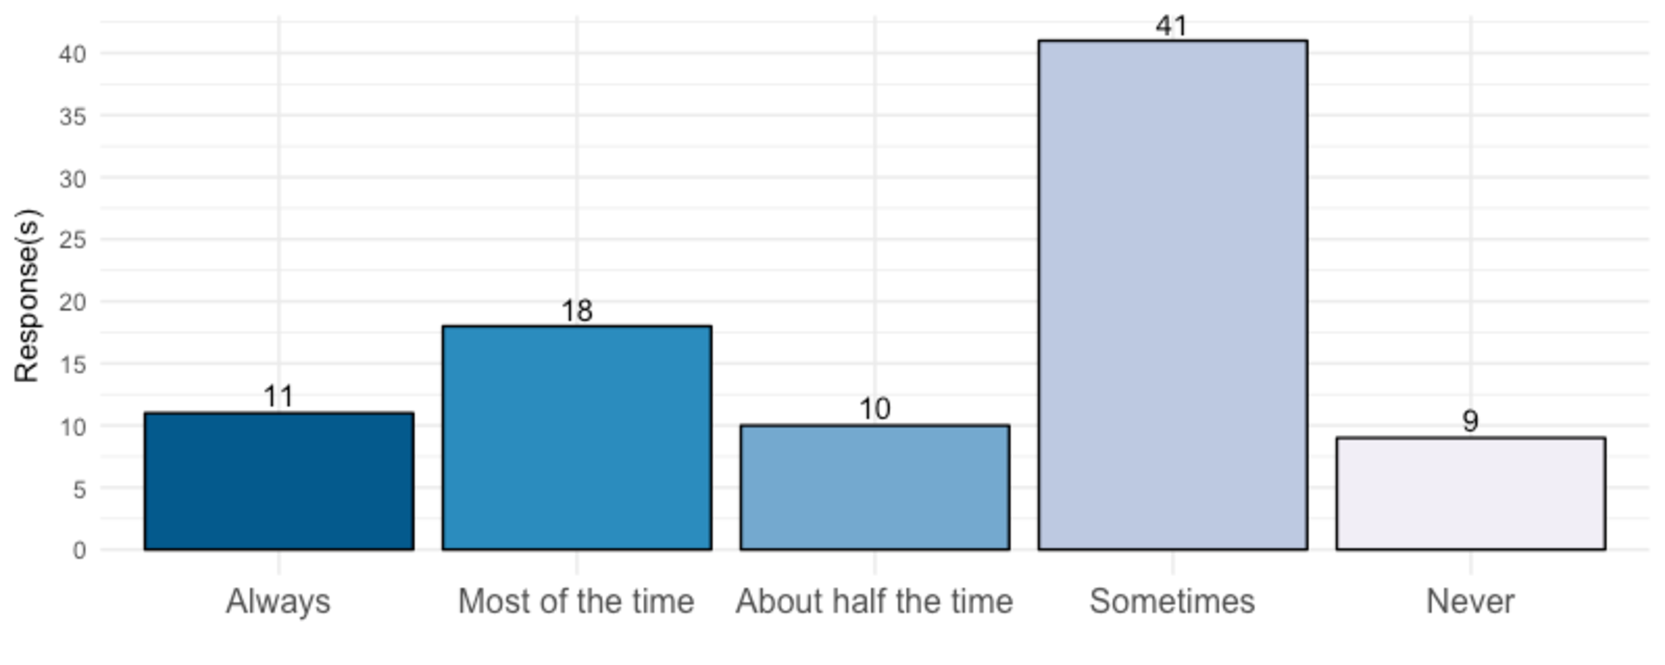
\includegraphics[width=0.98\textwidth,keepaspectratio]{imgs/CodeOwnershipFactor}}
%\caption{Degree of Code Ownership as a Factor in Merge Conflict Strategies. Scale: 1 is \textit{Always} and 5 is \textit{Never}. 89 out of 102 participants (87.26\%) provided a response to this question in the \textit{Processes Survey}~(S1).\vspace*{-0.3\baselineskip}}
%\label{fig:code-ownership-resolution}
%\end{figure}

To conclude, developers reported that expertise in the area of the conflicting code is one of the top factors in determining the difficulty of a merge conflict.
Additionally, developers also indicate that increases in perceived complexity of merge conflicts is strongly linked with the degree of difficulty in resolving them.
Therefore, developers' perceptions and intuition are relied on throughout the implementation of their resolution.

\nsubsection{Code Ownership in Merge Conflict Resolution Strategies}

\boldif{The role of code ownership in the resolution strategy.}
Finally, we found that, on average, participants indicate that code ownership factors \textit{about half the time} in their strategy of code ownership (mean: $3.21$ on a 5-point Likert-type scale).
This is consistent with their responses for their criteria for deferring a resolution, where it is the third most common factor in their decision. 
Only 10.11\% of participants indicated that code ownership \textit{never} factors into their resolution strategy (see Figure~\ref{fig:code-ownership-resolution}).

\subsubsection{\textbf{RQ1c}: How do software developers \textbf{evaluate} merge conflict resolutions?}\label{RQ1c}

After implementing a merge conflict resolution, software developers must evaluate whether their resolution has returned the codebase to a clean state.
We asked developers to select the conditions (from interviews) that they use to determine whether their resolution has successfully addressed the merge conflict.

\nsubsection{Success Conditions for Merge Conflict Resolutions}

In the \textit{Exploratory Interviews}, developers described six common conditions they considered important in their evaluation.
We asked \textit{Processes Survey}~(S1) participants to select from this list of conditions, including an \textit{Other} option to elicit additional conditions.
Only two developers selected that condition, indicating ``performance tests showing similar performance'' and ``client approval.''
We received 324 selections from 89 participants and present the aggregated results in Table~\ref{conditionsSuccess}.

\begin{table}[!htbp]
\caption{Conditions of Successful Merge Conflict Resolutions from Processes Survey (S1)\textsuperscript{i}}
\label{conditionsSuccess}
\centering
\begin{tabularx}{\textwidth}{@{}lr|*{7}{C}c@{}}
\toprule
	&
	& C1
	& C2
	& C3
	& C4
	& C5
	& C6
	& C7 \\
\midrule
	C1 & All tests pass & \textbf{67} & & & & & & \\
	C2 & Code compiles & 50 & \textbf{67} & & & & & \\
	C3 & Code looks correct & 50 & 54 & \textbf{66} & & & & \\
	C4 & VCS warmings gone & 38 & 42 & 41 & 51 & & & \\
	C5 & Code reviewed & 32 & 31 & 27 & 25 & 38 & & \\
	C6 & Merged to production & 27 & 27 & 27 & 26 & 19 & 33 & \\
	C7 & Other & 2 & 2 & 0 & 0 & 0 & 0 & 2 \\
\bottomrule
    \multicolumn{9}{c}{\noindent\parbox[t]{11.7cm}{\vspace{0.4em}\textsuperscript{i}\hspace{0.2em}\textit{Processes Survey}~(S1) participants were allowed to select multiple conditions. Each entry represents the number of participants that selected both of the conditions indicated for the column and row. 68 out of 102 participants (67\%) selected three or more conditions.}\vspace*{-0.3\baselineskip}} \\
\end{tabularx}
\end{table}

\textit{All tests pass} (C1), \textit{code successfully compiles} (C2), and \textit{code looks correct (i.e. visual test passes)} (C3) were the most commonly selected conditions required for a successful merge resolution.
These results are in line with existing literature showing that testing (C1) can be used for validating program functionality and correctness~\cite{beizer1984software,tian2005software}. %and have been fundamental to development processes such as test-driven development for several years~\cite{beck2003test}.
Similarly, the use of compilers to validate code (C2) as being executable and in good-working order will be familiar to any developer using a compiled programming language.

The use of visual inspection as a measure of successful merge conflict resolutions is surprising to us, given that \textit{complexity of conflicting lines of code}~(F1) is the highest rate factor for impact on merge conflict difficulty~\cite{mckee2017software}.
Inspecting code requires time and expertise in the area of conflicting code.
However, the survey participants that selected \textit{code looks correct (i.e. visual test passes)}~(C3) had a mean of 9.2 years of programming experience, which is only slightly higher than the overall mean of 9.0 years of programming experience.

Looking at the combination of \textit{code looks correct (i.e. visual test passes)}~(C3) with the other conditions, we find that 54 participants also selected \textit{all tests pass}~(C1) (52.9\%).
As the most common co-occuring selections, we conclude that although developers rely upon their expertise to visually inspect a merge conflict resolution, they also run the test suite to validate their evaluation.
Experience can play a big factor, as this method (C3) is highly subjective.

\boldif{Tests are still the most common criteria for determining a merge conflict resolution successful.}
The two most common evaluation criteria that developers mentioned are that the \emph{code compiles,} and that \emph{all tests pass.}
However, less then half selected both options.
While tests passing can be considered a good criteria of a successful resolution, the fact that the code compiles is not.
Even if the code compiles, there can be logical errors that are introduced during the merge resolution process, especially if the resolution was difficult.

\boldif{Only a minority of developers mention that code review is part of their success criteria}
Interestingly, only a minority of developers (37.25\%) mentioned code reviews as part of their success criteria.
%TODO add citation for the code review part
While code reviews are an effective way to detect bugs introduced by changes in the codebase, the practice appears to have not been adopted for code changed during merge conflict resolutions.

\nsubsection{Merge Resolution Evaluation Toolsets}

From the \textit{Exploratory Interviews}, we identified five categories of software development tools that developers mention in relation to merge conflicts.
In the \textit{Processes Survey}~(S1), we asked the developers to identify the tools they use when evaluating a merge conflict resolution.
We received 204 selections from 89 participants.
The aggregated results are presented in Table~\ref{resolution-evaluation-tools}, ranked according to the percentage of participants that selected each toolset.

\begin{table}[!htbp]
\renewcommand{\arraystretch}{1.2}
\caption{Merge Resolution Evaluation Toolsets from Processes Survey (S1)}
\label{resolution-evaluation-tools}
\centering
\begin{tabularx}{\textwidth}{>{\rowmac}l | >{\rowmac}c | >{\rowmac}r <{\clearrow}}
\toprule
  \parnoteclear % tabularx will otherwise add each note thrice
  Description & \# Selections\parnote{\textit{Processes Survey}~(S1) participants were allowed to select multiple toolsets. 64 out of 89 participants (71.91\%) selected multiple toolsets.\vspace*{-0.3\baselineskip}} & Percentage (\%)\textsuperscript{i} \\
\midrule
  Version Control Systems (e.g. Git, Subversion, CVS) & 82 & 92.14\% \\
  Continuous Integration (e.g. TravisCI, Jenkins, TFS) & 62 & 69.66\% \\
  Program Analysis Tools (e.g. Coverity, CodeSonar) & 26 & 29.21\% \\
  DevOps Tools (e.g. Nagios, Monit, Kabana) & 17 & 19.10\% \\
  Release Management Tools (e.g. Chef, Puppet, Salt) & 9 & 10.11\% \\
  Other Tools & 8 & 8.99\% \\
\bottomrule
\end{tabularx}
\parnotes
\end{table}
\vspace{0.8em}

By far, the most selected tools were \textit{version control systems} (VCS) and \textit{continuous integration} (CI) platforms, with 82 (92.14\%) and 62 (69.66\%), respectively.
The mean for all other tool categories was 15 selections (16.85\%), and represents a combined 29.4\% of response selections.

The use of version control systems to determine whether a resolution was successful aligns with the \textit{VCS warnings are gone} (C3) condition.
Also, continuous integration is dependent on code being compilable (C2), and tests being written and maintained (C1).
However, the availability of tools for evaluating merge conflict resolutions might constrain the conditions that developers are willing to consider for their merge conflict resolutions to be successful.
Further research is needed to determine whether there is a causal relationship between these dimensions, and whether more effective conditions could be supported by merge conflict toolsets.

\boldif{Some approaches will only detect direct merge conflicts, not indirect ones.}
Not all of the tools developers use for evaluating the result of a merge conflict resolution can detect all types of merge conflicts.
For example, Version Control Systems will detect only direct conflicts.
Even if the conflict is solved, from the version control systems' perspective, there still might be build or test issues.
Indirect conflicts might slip through if the developer does not run the test suite after resolving the conflict.
While almost 70\% of our participants mentioned that they used Continuous Integration as part of the evaluation process, those that don't might be inadvertently introducing bugs when they resolve the merge conflict.

\boldif{There is a lack of tool support that makes it difficult for developers to properly evaluate the success of a merge conflict resolution.}
Finally, developers have to manually check if their merge resolution is correct.
This is done, either by checking that the version control warnings are gone, inspecting the code for any mistakes, or by manually running the tests.
We notice that there is a lack of an automated process.
Without it the developer might, willingly or unwillingly, skip steps.
Also, this lack of a comprehensive toolset might hamper new developers in their efforts to successfully resolve merge conflicts.

\nsubsection{Backup Strategies}

Merge conflict resolutions are not always successful.
When they fail, developers must alter their patch and potentially switch strategies in order to successfully resolve the conflict.

To understand the prevalence of failed conflict resolutions, we asked \textit{Processes Survey}~(S1) participants to indicate the frequency in which their first attempt at resolving a merge conflict fails (see Figure~\ref{fig:first-attempt-failure}).
The most common response was \textit{somewhat infrequently} (mean: $3.49$ on a 5-point Likert-type scale).
This suggests that first attempts typically succeed.
However, this also shows that 78.7\% of participants (70 out of 89) occasionally fail at their first attempt and must make additional attempts to resolve a merge conflict.

\begin{figure}
	\centering
	\fbox{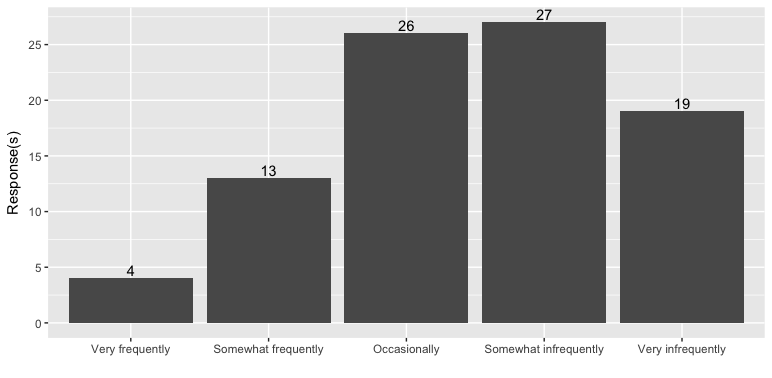
\includegraphics[width=0.95\textwidth,keepaspectratio]{FirstAttemptFailure}}
	\caption{Frequency of Failures in First Attempts at Merge Conflict Resolution. Scale: 1 is \textit{Very frequently} and 5 is \textit{very infrequently}. 89 out of 102 participants (87.26\%) indicated a frequency in the \textit{Processes Survey}~(S1).\vspace*{-0.3\baselineskip}}
	\label{fig:first-attempt-failure}
\end{figure}

Furthermore, we asked survey participants to describe their backup strategies when their first attempt at resolving a merge conflict fails.
We received 75 responses and the aggregate results are presented in Table~\ref{backup-strategies}, ranked according to the percentage of participants that described using each backup strategy.

Developers' backup strategies include \textit{take it offline} (B1), \textit{collaborating} (B2), \textit{try again} (B3), \textit{redoing changes} (B4), and \textit{no backup strategy} (B5).
Since \textit{no backup strategy} (B5) is not a strategy in and of itself, we focus on strategies B1--B4 instead.

The \textit{take it offline} (B1) strategy involves moving conflicting code away from shared branches or code repositories, and working locally to resolve the conflict without disrupting other developers.
The antithesis of this strategy is \textit{collaborating} (S2), where developers seek out other developers that are more knowledgeable about the area of conflicting code.
The B1 and B2 strategies contrast each other, and show that developers reserve more costly strategies (in terms of time, effort, and coordination) as backups to their primary resolution strategies.
The most common backup strategies, are in a way, opposite of the primary strategies.

Additionally, we find that developers also simply \textit{try again} (B3) to merge the same code together and hope that their tools are able to succeed with a second attempt.
Developers also resort to \textit{redoing changes} (B4), by way of reverting and manually recreating the changes found in conflicting commits when their initial attempt failed.
The B3 and B4 strategies appear to cement the extremes of the cost spectrum of backup strategies for resolving merge conflicts.
Simply retrying the same merge (B3) requires very little additional work.
It implies that developers think that they might have missed something, and that by going through the changes again, they might catch or have a better understanding of the two changes that are conflicting.
However, the process of redoing changes (B4) is a duplication of previous efforts. %and is therefore costly on developer's time.
This \textit{Nuclear Option} is clearly a time-consuming strategy for developers (both in planning and implementing a resolution), and yet the perceived costs of trying to unravel the conflicting code appear to be higher than the costs of reimplementing features.

\begin{table}[!htbp]
\renewcommand{\arraystretch}{1.2}
\caption{Backup Strategies for Resolving Merge Conflicts from Processes Survey (S1)}
\label{backup-strategies}
\centering
\begin{tabularx}{\textwidth}{c|l|c|r}
\toprule
  \parnoteclear % tabularx will otherwise add each note thrice
  Strategy & Description & \# Participants\parnote{75 out of 102 participants (73.53\%) provided a description of their backup strategy.\vspace*{-0.3\baselineskip}} & Percentage (\%)\textsuperscript{i} \\
\midrule
  B1 & Take it offline & 19 & 25.33\% \\
  B2 & Collaborating & 17 & 22.67\% \\
  B3 & Try again & 15 & 20.00\% \\
  B4 & Redoing changes & 14 & 18.67\% \\
  B5 & No backup strategy\hspace{2.0cm} & 10 & 13.33\% \\
\bottomrule
\end{tabularx}
\parnotes
\end{table}
\vspace{0.8em}

\boldif{Some developers do not have an approach for dealing with merge conflicts.}
Finally, an interesting result is that some developers do not have a strategy for approaching a merge conflict resolution.
The existence of this \textit{no strategy} approach is anecdotal, but curious, since we assume that developers are rational actors seeking to organize themselves in ways that increase the likelihood of successful outcomes.
Yet this strategy appears to go counter to that notion.
One explanation for the lack of a strategy is the lack of experience.
With a mean of 3.5 years of programming experience (5.6 years less than the overall mean), these participants might not have encountered enough situations to form a coherent strategy.

Interestingly, when developers perceive a merge conflict to be too difficult to resolve they occasionally resort to removing all conflicting code and reimplementing the underlying functionality in order to fix it.

%!TEX root = main.tex

\subsection{\textbf{RQ2:} What difficulties do software developers experience when managing merge conflicts?}\label{RQ2}

To understand the difficulties for software developers when encountering a merge conflict, we asked interview participants to reflect on situations when they initially face a merge conflict: what kind of information do they seek, how do they approach the resolution of the conflict, and what tools do they use. 

\subsubsection{Difficulty Factors}\label{difficulty-factors}

From the card sorting of the interview answers (Section~\ref{interviews}), we identified nine factors that developers consider when approaching a conflict and attempting to determine its difficulty (see Table~\ref{s2_factors}). 
We asked \textit{Barrier Survey}~(S2) participants to rate how each of these nine factors affected their perceptions of difficulty when approaching a merge conflict.

We received 162 responses and present the aggregated results in Table~\ref{s2_factors}; ranked according to the mean score for each factor.
Here, we discuss in detail the top 4 factors with a mean score greater than $3.00$.
These factors can be grouped into themes of \textit{technical aspects} and \textit{expertise,} and our results are presented according to these groups.

\begin{table}[!htbp]
\renewcommand{\arraystretch}{1.2}
\caption{Difficulty Factors of Merge Conflicts from Barriers Survey (S2)}
\label{s2_factors}
\centering
\begin{tabularx}{\textwidth}{>{\rowmac}c | >{\rowmac}l | *1{>{\rowmac}c} | *2{>{\rowmac}c}<{\clearrow}}
\toprule
  \parnoteclear % tabularx will otherwise add each note thrice
  Factor & Description & \likertscale{1,2,3,4,5} & Median\parnote{Responses on 5-point Likert scale indicating the degree of effect on resolution difficulty (1 indicates \textit{no effect}, 5 indicates \textit{great effect}).} & Mean\textsuperscript{i} \\
\midrule
  \setrow{\bfseries}F1 & Complexity of conflicting lines of code & \likertplot{coordinates {(1,5)(2,29)(3,38)(4,56)(5,34)}}{28.2}{5,29,38,56,34} & 4 & 3.52 \\
  \setrow{\bfseries}F2 & Expertise in area of conflicting code & \likertplot{coordinates {(1,5)(2,23)(3,50)(4,54)(5,30)}}{28.2}{5,23,50,54,30} & 4 & 3.50 \\
  \setrow{\bfseries}F3 & Complexity of files with conflicts & \likertplot{coordinates {(1,8)(2,34)(3,49)(4,51)(5,18)}}{28.2}{8,34,49,51,18} & 3 & 3.23 \\
  \setrow{\bfseries}F4 & Number of conflicting lines of code & \likertplot{coordinates {(1,2)(2,40)(3,64)(4,45)(5,11)}}{28.2}{2,40,64,45,11} & 3 & 3.14 \\
  F5 & Time to resolve a conflict & \likertplot{coordinates {(1,14)(2,56)(3,51)(4,25)(5,15)}}{28.2}{14,56,51,25,15} & 3 & 2.82 \\
  F6 & Atomicity of changesets in conflict & \likertplot{coordinates {(1,20)(2,48)(3,51)(4,29)(5,13)}}{28.2}{20,48,51,29,13} & 3 & 2.80 \\
  F7 & Dependencies of conflicting code & \likertplot{coordinates {(1,20)(2,56)(3,39)(4,33)(5,14)}}{28.2}{20,56,39,33,14} & 3 & 2.78 \\
  F8 & Number of files in the conflict & \likertplot{coordinates {(1,10)(2,69)(3,50)(4,26)(5,6)}}{28.2}{10,69,50,26,6} & 3 & 2.68 \\
  F9 & Non-functional changes in codebase & \likertplot{coordinates {(1,47)(2,63)(3,31)(4,15)(5,4)}}{28.2}{47,63,31,15,4} & 2 & 2.16 \\
\bottomrule
\end{tabularx}
\parnotes
\end{table}

\nsubsection{Technical Aspects}\label{artifact-based-factors}
Two of the top four factors refer to the perceptions about the complexity of merge conflicts (F1, F3), with the third factor being \textit{number of conflicting lines of code} (F4), which can be construed as a specific metric for the complexity of the conflict. 
While developers mentioned complexity of the lines of code and the file, none mentioned using any metrics, such as cyclomatic complexity~\cite{fenton2000quantitative,mccabe1976complexity}, Function Point Analysis~\cite{garmus2001fpa,symons1988function} etc. 
Instead, developers made educated guesses on the complexity of the code based on their own experience of either writing the code, or having worked with it. 
Some of the simple to compute metrics, such as \textit{number of conflicting lines of code} (F4), \textit{number of files in the conflict} (F8), \textit{atomicity of changesets in conflict} (F6), and the \textit{time to resolve a conflict} (F5) were mentioned. 
The only factor where static analysis tools can help was in identifying the \textit{dependencies of conflicting code} (F7).
This indicates that understanding the complexity of the conflicting code is important, but developers do not use the metrics that have been proposed by research.
While some of the simple proxies for complexity are used, developers primarily rely on their own judgement of the complexity of a conflict.

This perception of the conflict complexity can affect whether a developer resolves the conflict immediately (when small), or whether they should wait to examine the conflict when further resources are available; P8 commented:
\begin{quoting}
\textit{``Small is always easy. A 1-line merge conflict is always easier to resolve than a 400-line merge conflict, and can be done now.''}
\end{quoting}

If a merge conflict is perceived to be large or complex, a developer may decide to forgo attempting to resolve it through code manipulation and choose to revert the changes instead~\cite{Guzzi2015}.
This ``nuclear option'' requires developers to disrupt the development flow, set aside their current development work, and potentially remove good, working code that was not part of the conflict in order to return to a non-conflicting state.
In the interview, P1 describes this process as:
\begin{quoting}
\textit{``If you have many conflicts involved, many commits in the conflict...throw one of the branches away. You cannot combine tens of commits conflicting...it's not sane!''}
\end{quoting}

Further, when integrators are preparing code for production environments they prioritize merge conflicts for code review based upon the perceived difficulty of resolving the affected code.
We find that these decisions rely on human judgement factors as much as they rely on data-driven metrics.
Developers may not have the time to compute project-wide complexity metrics, such as those proposed in  literature.
Therefore, we need metrics that can be easily calculated by unexperienced developers as they face a conflict. 
%are human-aware and take into account the perceived difficulties of merge conflicts.

\nsubsection{Expertise}\label{knowledge-based-factors}
Our findings show that \textit{expertise in the area of conflicting code}~(F2) is one of the top factors in determining the difficulty of a merge conflict. 
This reiterates the fact that developers rely on their own knowledge about the conflicting codebase when approaching a conflict. 
And as seen in Section~\ref{RQ1c}, this expertise has a direct impact on the ability of developers to use \textit{code looks correct (i.e. visual test passes)} (C3) as a strategy for evaluating merge conflict resolutions.

Our results indicate that when developers feel they don't have the expertise in the conflicting codebase, they consider the conflict difficult to merge and seek out more information or assistance from others.
P5 illustrated this need for expertise when describing his workflow: 
\begin{quoting}
	\textit{``A lot of what I work on is in my own little area \textellipsis I know what to do [\textellipsis]. But in [unfamiliar part of code,] then I'll get someone else to resolve the merge conflict for me. It's someone else's code, and I don't want to screw it up.''}
\end{quoting}

Our findings confirm the need for tools that identify appropriate experts~\cite{CostaSarma} and encourage further research into selection of knowledgeable developers for merge conflict resolution.

%%%%%%%%%%%%%%%%%%%%%%%%%%%%%%%%%%%%%%%%%%%%%%%%%%%%%%%%%%%%%%%%%

%\subsubsection{Interviews}
%%The interview results suggest that developers approach merge conflicts...
%
%\subsubsection{Survey}
%Our survey suggests that regardless of gender, developer role, experience level, project size, and source distribution model, software practitioners say that the following factors affect the difficulty of a merge conflict most: 
%\begin{itemize}
%\item \textit{Complexity of conflicting lines of code}
%\item \textit{Your knowledge/expertise in area of conflicting code}
%\end{itemize}
%
%Similarly, software practitioners across every measured demographic perceived the following factors to be less important when deciding the difficulty of a merge conflict:
%\begin{itemize}
%\item \textit{Non-functional changes (whitespace, renaming, etc)}
%\item \textit{Number of files in the conflict}
%\end{itemize}
%
%While survey participants did not agree that non-functional changes strongly factor into the difficulty of a merge conflict, it is still worth noting that several interview participants named non-functional changes, such as large refactor or reformatting changes, as a cause for merge conflicts. This suggests that non-functional changes may increase the likelihood of a merge conflict happening, but they do not contribute to the conflict's difficulty.
%
%However, some demographics do view certain difficulties. For instance, open-source developers think that \textit{Atomicity of change sets in the conflict} impacts the difficulty, while closed-source developers and people who split their time evenly think that atomic change sets have no effect on the difficulty. This may be explained by the findings in Rigby et al\cite{OSS_smaller_commits}, which shows that open-source projects tend to review smaller changes than closed-source projects because "The small size lets reviewers focus on the entire change, and the incrementality reduces reviewers’ preparation time and lets them maintain an overall picture of how the change fits into the system." It is possible that our result reflects this difference of culture.
%
%We also found that Project Maintainers say that \textit{Time to resolve a conflict} has an effect, while no other role agrees. This suggests that those in a maintainer role may be more subject to time-related constraints such as maintenance or release schedules. 
%
%\comment{Project Managers say no effect because they focus on project schedules, not conflict resolutions, i.e. they are higher level/abstraction?}
%
%\todo{might be previous work}
%Support and infrastructure roles (System Engineer, Sys Admin, System Architect, DevOps) emphasized that \textit{Dependencies of conflicting code on other components} have more of an effect than other roles did. This might be due to infrastructure systems being maintained in a live environment, or systems that are currently in production use and at risk of real-time dependency failures. 
%
%Developers on projects of size 1 say that \textit{Dependencies of conflicting code on other components}. Because no other project sizes agree with this idea, we hypothesize that this could be due to their high dependence on external code because of the software production limitations of a 1-developer team.
%
%We also found that the group of developers with 21-25 years of experience frequently contradicted general consensus, but it seems more likely that these differences were simply due to the group's small sample size (4).

%We asked participants how much they trust their merging, history exploration, and/or conflict resolution tools, and 57.9\% of participants reported that they trusted these tools either \textit{A Lot} or \textit{Completely}. While this is a majority of developers, this still leaves a significant number of people (42.1\%) who trust their tools \textit{A moderate amount} or \textit{A little}. Though we had the option for \textit{Not at all}, no participants selected this option, presumably because users stop using tools that they do not trust at all. While we found no previous work discussing the threshold for how much users must trust tools for a good tool experience, we postulate that users who cannot trust their tools \textit{A Lot} or \textit{Completely} will avoid relying on such tools too much.

%\subsubsection{\textbf{Old RQ3:} What unmet needs impact the difficulty of merge conflict resolutions?}

\subsubsection{Unmet Needs for Merge Conflict Resolutions}

There can often be gaps in how developers perceive the difficulty of merge conflicts and the actual hurdles that they face when resolving these conflicts. 
These gaps can then in turn affect how effective developers are at resolving the conflict.

We, therefore, asked our interview participants open-ended questions about their experiences in resolving the most recent conflicts, especially their recollection of what made the resolution difficult.
Their responses indicated that there are several unmet needs.
We identified ten needs (see Table~\ref{s2_needs}), which range from needs about the ability to understand the code, their expertise, and existing tool support.  

\begin{table}[!htbp]
\renewcommand{\arraystretch}{1.2}
\caption{Developer Needs for Merge Conflict Resolutions from Barriers Survey (S2)}
\label{s2_needs}
\centering
\begin{tabularx}{\textwidth}{>{\rowmac}c | >{\rowmac}l | *1{>{\rowmac}c} | *2{>{\rowmac}c}<{\clearrow}}
\toprule
  \parnoteclear % tabularx will otherwise add each note thrice
  Need & Description & \likertscale{1,2,3,4,5} & Median\parnote{Responses on 5-point Likert scale indicating the degree of importance to merge resolutions (1 indicates \textit{no importance}, 5 indicates \textit{great importance}).} & Mean\textsuperscript{i} \\
\midrule
  \setrow{\bfseries}N1 & Ease of understanding conflicting code & \likertplot{coordinates {(1,0)(2,14)(3,25)(4,65)(5,37)}}{28.2}{0,14,25,65,37} & 4 & 3.89 \\
  \setrow{\bfseries}N2 & Expertise in area of conflicting code & \likertplot{coordinates {(1,1)(2,17)(3,38)(4,49)(5,36)}}{28.2}{1,17,38,49,36} & 4 & 3.72 \\
  \setrow{\bfseries}N3 & Amount of info about conflicting code & \likertplot{coordinates {(1,2)(2,21)(3,38)(4,48)(5,32)}}{28.2}{2,21,38,48,32} & 4 & 3.62 \\
  \setrow{\bfseries}N4 & Tools presenting understandable info & \likertplot{coordinates {(1,4)(2,24)(3,47)(4,32)(5,34)}}{28.2}{4,24,47,32,34} & 3 & 3.48 \\
  N5 & Changing assumptions within code & \likertplot{coordinates {(1,8)(2,27)(3,45)(4,36)(5,25)}}{28.2}{8,27,45,36,25} & 3 & 3.30 \\
  N6 & Complexity of project structure & \likertplot{coordinates {(1,6)(2,38)(3,39)(4,41)(5,17)}}{28.2}{6,38,39,41,17} & 3 & 3.18 \\
  N7 & Trustworthiness of tools & \likertplot{coordinates {(1,17)(2,29)(3,39)(4,32)(5,34)}}{28.2}{17,29,39,32,34} & 3 & 3.12 \\
  N8 & Informativeness of commit messages & \likertplot{coordinates {(1,18)(2,32)(3,30)(4,44)(5,17)}}{28.2}{18,32,30,44,17} & 3 & 3.07 \\
  N9 & Project culture & \likertplot{coordinates {(1,13)(2,37)(3,43)(4,27)(5,21)}}{28.2}{13,37,43,27,21} & 3 & 3.04 \\
  N10 & Tool support for history exploration & \likertplot{coordinates {(1,16)(2,40)(3,31)(4,32)(5,22)}}{28.2}{16,40,31,32,22} & 3 & 3.03 \\
\bottomrule
\end{tabularx}
\parnotes
\end{table}

Using results from the interview, we asked S2 survey participants to rate how much each of the ten needs affected their ability to resolve the merge conflicts.
We received 141 responses using a 5-point Likert-type scale indicating the degree of effect on resolution difficulty (1 being \textit{Not at all}, 3 being \textit{A moderate amount}, and 5 being \textit{A great deal}).
Results of the survey are presented in Table~\ref{s2_needs}. 

All the unmet needs have a mean score of at least $3.03$ on the 5-point Likert-type scale, implying that all of them mattered at least a moderate amount.
We present and discuss in detail the top four unmet needs, plus additional observations regarding the other six unmet needs. 
As with the factors in the previous section, all these needs also relate to \textit{technical aspects} (e.g., understanding the conflicting code) and their \textit{expertise} in resolving conflicts.

%All of the unmet needs in Table~\ref{survey_res_diffs} can be considered important to practitioners when resolving merge conflicts, since each received a mean score of at least 3.03 on the 5-point Likert scale.
%However, practitioners primarily working on closed-source development differed in perceptions of \textit{tool support for examining development history} (N10).
%We further discuss this demographic difference in Section~\ref{oss_vs_closed_tool_support}.

\nsubsection{Technical Aspects}
Three needs among the top four relate to technical aspects of merge conflict resolution.
The \textit{understandability of conflicting code} (N1) is ranked as the most important need, with both \textit{contextual information about the conflict} (N3) and \textit{the way in which tools present relevant information} (N4) ranking in the top four.

Data from version control systems is used by developers to identify the evolution of the code~\cite{Mihai_lenses}, however, it is not easily available and requires a context switch from the code editor to the version control system~\cite{Guzzi2015}. 
Moreover, these changes are often processed in isolation, especially when there are many changes (conflicts) to process. 
Such decomposition of overall conflicting changes into smaller ``chunks" is needed to be able to manage the complexity of the resolution process; however, this occludes viewing the changes in a larger context. 
Often developers deal with the decomposed (smaller) changes, hoping that they will all together work out. 
For example, P1 compared the resolution hurdles between two conflicts, where one was simple, and the other spanned multiple files and complex blocks of code.
\begin{quoting}
\textit{``You focus on understanding the small change, not the big one. It's easier to understand... get the small change to go with the flow of the bigger change.''}
\end{quoting}

Another challenge when viewing changes in isolation, is the fact that developers may miss the impact of the changes made as part of the resolution to the rest of the code base. 
Identifying the impact of changes on the rest of the code base has been repeatedly found to be a problem in collaborative development, as found by deSouza and Redmiles~\cite{deSouza2008} and more recently by Guzzi et al.~\cite{Guzzi2015}. 
The top unmet needs in our study also revolved around the challenges that developers face in how much information they had about the conflicting code (N3), and the difficulty in finding the needed information from current tools and practices (N3, N4, N8, N10). 
This indicates that despite advances in supporting parallel development practices, the right information needed to resolve conflicts is still not easily available to developers. 

Conflict resolution can sometime lead to defects in the code base. This can arise because of several reasons. For example the rationale of the two conflicting changes might be unclear and the merge might cause unintentional problems down the line. Or the resolved changes might not follow rigorous code review and testing to which the original changes were subject to.
Therefore, even when the practitioner understands the particular conflicting code, they may still need additional meta information about the rationale of changes and idea of future feature implementation. This is especially true in situations where the code base is old, and such information not readily available. During our interview, P7 commented:
\begin{quoting}
\textit{``It's harder to merge code when you're merging in some legacy code... But if you're a young team, and everybody who wrote the code is still a part of the team, it's easier.''}
\end{quoting}

\nsubsection{Expertise}
Knowledge is a key component of developer's needs when resolving merge conflicts, but along with that general knowledge is a need for expertise in the specific areas of code involved in a conflict.
Developers recognize this need as having a sizable effect on their ability to resolve a merge conflict, and selected \textit{expertise in the area of conflicting code} (N2) as the second most important need.

Examining code artifacts, reviewing change history, and reading documentation help with understanding the code when they are present and well-maintained.
However, locating and maintaining these supporting documents is not always possible.
In fact, Forward et al.~\cite{forward2002documentation} conducted a survey of 48 software developers and found that 68\% either agreed or strongly agreed that documentation is always outdated.
When these gaps arise, developers compensate by consulting experts in the area of conflicting code instead.

This result aligns with the goals of the TIPMerge tool~\cite{CostaSarma}, which seeks to locate experts that are best suited to resolve conflicts in a particular area of code.
However, TIPMerge, as well as other recommendation tools are not being used by real-world developers, as evidenced by the lack of such tools in the list of top 10 merge resolution tools (see Table~\ref{s2_toolset}).
The reason for this lack of research tools adoption requires further investigation.

Another surprising fact was that while the informative nature of commit messages (N8) and project culture (N9) were mentioned, they were not as highly ranked. % The same is true for project culture (N9). 
We had expected them to be higher based on prior work~\cite{yamauchi2014clustering, hindle2009automatic, cortes2014automatically, hattori2008nature}. 
We found no statistical differences between commercial or open source projects, including when accounting for experience levels.
Our results indicate that team practices, including writing commit messages may have matured enough, such that these factors are no longer considered critical in our sample set. 


%\nsubsection{Open-Source vs. Closed-Source Needs}\label{oss_vs_closed_tool_support} 
%It is interesting to note that for needs N1-N8 there was no statistical difference between practitioners focused on open-source and those focused on closed-source development when it comes to their conflict resolution needs.
%We found that practitioners who focus on open-source software development consider \textit{tool support for examining development history} (N10) to be the 3rd highest unmet need (mean: 3.60).
%Whereas, practitioners who focus on closed-source software development consider it to be the least impactful unmet need (mean: 2.86).
%%A Wilcoxon Signed-Ranks test indicated that open-source practitioners' ranking of N10 were statistically higher than closed-source practitioners' rankings of N10 (W = 1192.5, $p$-value = 0.02).
%
%This was also true in our interviews, with P8 stating:
%
%\begin{quoting}
%\textit{``I'm often dealing with code other people wrote. Nobody can review every pull request. So now I have to go back and do some archaeology to find out what's going on. Code is much easier to write than read.''}
%\end{quoting}
%
%This result suggests that history exploration in open-source projects is a more difficult task due to the lack of upfront planning and large number of volunteering contributors.
%%, or that tools are better at supporting history exploration in closed-source development environments.
%!TEX root = main.tex

\subsection{\textbf{RQ3:} How well do tools support developer's needs for managing merge conflicts?}\label{RQ3}

\begin{table}[!htbp]
\renewcommand{\arraystretch}{1.2}
\caption{Desired Improvements to Merge Toolsets from Barriers Survey (S2)}
\label{s2_tool_improvements}
\centering
\begin{tabularx}{\textwidth}{>{\rowmac}c | >{\rowmac}l | *1{>{\rowmac}c} | *2{>{\rowmac}c}<{\clearrow}}
\toprule
  \parnoteclear % tabularx will otherwise add each note thrice
  Imp.\parnote{Imp. = Improvement} & Description & \likertscale{1,2,3,4,5} & Median\parnote{Responses on 5-point Likert scale indicating the degree of potential impact on merge conflict processes (1 indicates \textit{no impact}, 5 indicates \textit{great impact}).} & Mean\textsuperscript{ii} \\
\midrule
  \setrow{\bfseries}I1 & Usability & \likertplot{coordinates {(1,6)(2,17)(3,32)(4,48)(5,16)}}{28.2}{6,17,32,48,16} & 4 & 3.43 \\
  \setrow{\bfseries}I2 & Filtering of relevant information & \likertplot{coordinates {(1,8)(2,15)(3,32)(4,48)(5,16)}}{28.2}{8,15,32,48,16} & 4 & 3.41 \\
  \setrow{\bfseries}I3 & Support for exploring project history & \likertplot{coordinates {(1,7)(2,21)(3,36)(4,39)(5,16)}}{28.2}{7,21,36,39,16} & 3 & 3.30 \\
  \setrow{\bfseries}I4 & Graphical information presentation & \likertplot{coordinates {(1,13)(2,26)(3,26)(4,37)(5,16)}}{28.2}{13,26,26,37,16} & 3 & 3.14 \\
  I5 & Transparent tool functionality/operations & \likertplot{coordinates {(1,16)(2,36)(3,24)(4,40)(5,3)}}{28.2}{16,36,24,40,3} & 3 & 2.82 \\
  I6 & Terminology consistent with other tools & \likertplot{coordinates {(1,23)(2,41)(3,32)(4,15)(5,8)}}{28.2}{23,41,32,15,8} & 2 & 2.53 \\
\bottomrule
\end{tabularx}
  \parnotes
\end{table}

Development tools need to be easy to use and provide contextualized, pertinent information in a manner that is easy to understand.
To investigate how well current tools satisfy the needs of practitioners, we asked interview participants open-ended questions about how they resolve merge conflicts.
We also ask about improvements that would be most valuable to them. 

Our results indicate that practitioners use a wide range of tools, with many directly using the Git command line interface. Our interview participants mentioned six different dimensions along which they would like improvements to tool support (see Table~\ref{s2_tool_improvements}). 

We framed the survey questions to validate the improvement needs expressed in our interviews, and ranked those six needs according to mean score.
Table~\ref{s2_tool_improvements} presents the needs from the survey responses ordered by their mean scores.
We received 119 responses using a 5-point Likert-type scale to indicate the usefulness of each type of tool improvement (1 being \textit{Not Useful}, 3 being \textit{Moderately Useful}, and 5 being \textit{Essential}).

In addition, we also asked participants which tools they use during conflict resolution.
We identified 105 different tools from the 115 responses. Some mentioned generic responses such as \textit{`` text editor''}, for which we create a separate category.
%We group these generic responses together where semantically similar meanings exist. 
Table~\ref{s2_toolset} lists the top 10 most common tools used by participants to resolve merge conflicts.

In examining the list of these tools, we note that practitioners most often use basic tools (e.g. Git, Vim/vi, or a Text Editor) to handle merge conflicts instead of employing specialized tools or plugins to modern IDEs. 
In this list, there is only one IDE (Eclipse), and three diff/merge toolsets (Git Diff, KDiff3, and Meld). 
This indicates that practitioners are currently not leveraging the functionalities provided by many research prototypes (e.g., Palantir~\cite{palantir}, Crystal~\cite{Brun2011}) that are specifically designed to facilitate proactive conflict detection, since they are built as plug-ins to modern IDEs. 

We next discuss the top four improvements rated by survey respondents. These are the responses that have a mean value higher than $3.00$.

\begin{table}[!htbp]
\renewcommand{\arraystretch}{1.3}
\caption{Merge Resolution Toolsets (Top 10) from Barriers Survey (S2)}
\label{s2_toolset}
\centering
\begin{tabularx}{\textwidth}{ll|c}
\toprule
  \parnoteclear % tabularx will otherwise add each note thrice
  Tool & Description & \# Participants (\%)\parnote{
  Survey participants were allowed to provide multiple tools. Each entry represents the number (and percentage) of participants that responded with that particular tool. 115 out of 162 respondents (71\%) indicated the use of at least one merge resolution tool.}\\
\midrule
  Git & Version Control System & 37 (15.68\%)\\
  Vim/vi & Text Editor & 17 (7.20\%)\\
  Text Editor (unspecified) & Text Editor & 14 (5.93\%)\\
  Git Diff & Diffing Tool & 11 (4.66\%)\\
  GitHub & Website & 11 (4.66\%)\\
  Eclipse & IDE & 10 (4.24\%)\\
  KDiff3 & Diff \& Merge & 9 (3.81\%)\\
  Meld & Diff \& Merge & 8 (3.39\%)\\
  SourceTree & Git/Hg Desktop Client & 8 (3.39\%)\\
  Sublime Text & Text Editor\hspace{3.2cm} & 7 (2.97\%)\\
\bottomrule
\end{tabularx}
\parnotes
\end{table}

\subsubsection{Better Usability}
%The right toolset is essential for efficiently developing solutions and resolving conflicts.
Usability is an important factor that determines whether a toolset supports or hinders the practitioner's workflow.
Our survey results indicate that \textit{better usability} (I1) is the most desired improvement of toolsets used for conflict resolution. 
%Based on the results of the survey, we found that practitioners rate usability as the most desired improvement for their current merge tools (I1).
While usability of a particular tool is important, the usability concerns become even more pertinent when they span multiple tools that are similar and must operate in sync with each other.
Survey results indicate that participants use an average of 2.5 tools, and as many as 7 tools, to resolve merge conflicts.
%With multiple tools being used during merging and conflict resolution, toolset fragmentation is a real concern for practitioners.
For instance, in our interview P1 demonstrated how he typically resolved a merge conflict by using four different tools and said: 
\begin{quoting}
\textit{``I have to jump around between tools and copy and paste version numbers...this is why integration matters.''}
\end{quoting}

Switching across multiple tools while resolving a conflict is disruptive and comes at a cost. Psychology studies~\cite{Meiran2000}\cite{gopher2000switching} have shown that task switching reduces performance and causes mental fatigue. 
Gerald Weinberg highlighted that context switching arising from toolset fragmentation is a big problem in engineering teams~\cite{Weinberg1992}. 

%This frustration is understandable for practitioners whose workflows frequently get interrupted by tool switches. Psychology studies~\cite{Meiran2000}\cite{gopher2000switching} have found that task switching comes with costs in performance and mental fatigue, and, in 1992, Gerald Weinberg highlighted the problem of toolset fragmentation within engineering teams~\cite{Weinberg1992}. 

\subsubsection{Better Exploration of Project History}
Practitioners have been known to use historical data to understand code evolution and development processes~\cite{Mihai_lenses}.
Version control and bug tracking systems contain a huge amount of meta-information about the evolution of code and development processes.
However, it is not easy to find the right bit of information in these large systems. 
Currently, there is insufficient support for performing detailed analysis of how a code snippet evolved over time and why. 
Better ways of exploring the project history (I3) was one of the top requested improvements in our survey. 
As P1 mentioned in the interview:
\begin{quoting}
\textit{``Give me a way to explore the history. To drill down, to go back up, you know? To resurface and understand what happened.''}
\end{quoting}


Currently, when performing any complex analysis it is easier to write stand alone scripts to extract the information. 
During the interview, P1 mentioned that he has written several scripts to locate particular historical commits that relate to a current merge conflict. 
Similarly, P9 described a tool, \texttt{git-diff}, that was developed by their team to add additional difference analysis functionality across branches:
\begin{quoting}
\textit{``git-diff will just do the diff based on the SHAs... we're adding metadata... It also hooks into GitHub labels to do some more advanced heuristics.''}
\end{quoting}

While writing these scripts allows extraction of relevant data contextualized to the need, it also leads to a proliferation of multiple scripts that are written by individual practitioners and need to be maintained or integrated.
This further adds to the problem of context-switching when practitioners must switch between multiple tools, and execute multiple scripts.

We are not the first to recognize the gap in tool support provided for analyzing development history among practitioners~\cite{Mihai_lenses, sun2015informationhistory, guo2016cold-start, yan2014miningcontracts}. 
It appears that practical applications of history exploration are still beyond the reach of practitioners. 
One of the reasons for this might be the simple set of text editors, and toolsets, that our study participants seem to prefer.

\subsubsection{Better Filtering of Less-Relevant Information}\label{better_filtering}
Tools that routinely handle large or complex datasets require filtering in order to efficiently locate desired pieces of information.
For example, when there are several commits in a pull request and multiple levels of code review at the line level.
It is difficult to extract the key issue in the pull request, which can get lost in the sea of low level details. Similarly, if there are multiple commits in a pull request or branch, it is hard to extract the right information.
Therefore, tools that provide filtering can better assist practitioners in working with large amounts of metadata associated with the changes.
\textit{Better ways of filtering out less relevant information} (I2) was selected as the second most important need; P1 explained:
\begin{quoting}
\textit{``You want to extract the relevant commits. The ones that actually clash...you want to zoom in on them and understand just enough and don't waste time.''}
\end{quoting}

While improvements in history exploration (I3) will make project metadata more accessible, improvements in filtering for relevant metadata will allow practitioners to focus on the relevant parts of the code impacted by the merge conflict.

%Version control systems (VCS) and bug tracking systems provide insufficient support for detailed analysis of software evolution and information retrieval~\cite{fischer2003release_history}.
%For software practitioners using \texttt{git} and other VCS, it is often easier to write scripts that accommodate their particular information needs by augmenting the capabilities of the VCS.
%During the interviews, P1 described writing several scripts in order to locate particular historical commits that relate to a current merge conflict.
%P9 also described a tool, \texttt{git-diff}, developed as part of their efforts to add additional difference analysis functionality across branches:
%\begin{displayquote}
%\textit{``git-diff will just do the diff based on the SHAs... we're adding metadata and cherry picking, so the SHAs are always going to be changing... It also hooks into GitHub labels and uses the labels on the project to do some more advanced heuristics.''}
%\end{displayquote}
%\todo{Shane: This transition is a bit rough}
%In our survey results, we see that practitioners rank \textit{better ways of filtering out less relevant information} (I2) as the second highest improvement needed in modern merge toolsets.
%This suggests that further work is needed to bring these capabilities from single-purpose scripts into common toolsets used by all practitioners.
%
%\Subsubsection{Better Exploration of Project History}
%Codoban et al.~\cite{mihai_lenses} introduced the concept of the \textit{Archeology Lens} to describe examining old development history to retrieve lost knowledge and postulated that additional tool support was needed in this context.
%We also find that practitioners consider history exploration to be a major area of improvement for development toolsets.
%Among survey participants, \textit{better ways of exploring project history} (I3) ranked as the third most important improvement needed.
%During our interviews, P1 said: 
%
%\begin{displayquote}
%\textit{``Give me a way to explore the history. To drill down, to go back up, you know? To resurface and understand what happened.''}
%\end{displayquote}
%
%The gap in support for analyzing development history among practitioner toolsets has previously been recognized by researchers~\cite{sun2015informationhistory, guo2016cold-start, yan2014miningcontracts}, however practical application of these efforts appear to have not yet reached practitioners.

\subsubsection{Better Graphical Presentation of Information}
The usefulness of information is helped or hindered by the way in which it is presented to users.
In our survey results, we found that \textit{better graphical presentation of information} (I4) was ranked the fourth highest improvement needed (mean: 3.14).

In our interviews, several practitioners reported experiencing issues with inconsistent terminology, inconsistent visual metaphors (e.g. colors, notifications, etc.), and the organizational layout of different development tools.
The cost of context switching in software development is well-known to researchers~\cite{czerwinski2004taskswitching, li2007cost_of_context_switch, blackwell2002attentioninvestment, convertino2003dualview}, and our results indicate that switching between different terminology and information presentation styles can also be a problem.
There is a need for tools that share commonality in both terminology and presentation. 

%\begin{figure*}[!htbp]
%\centering
%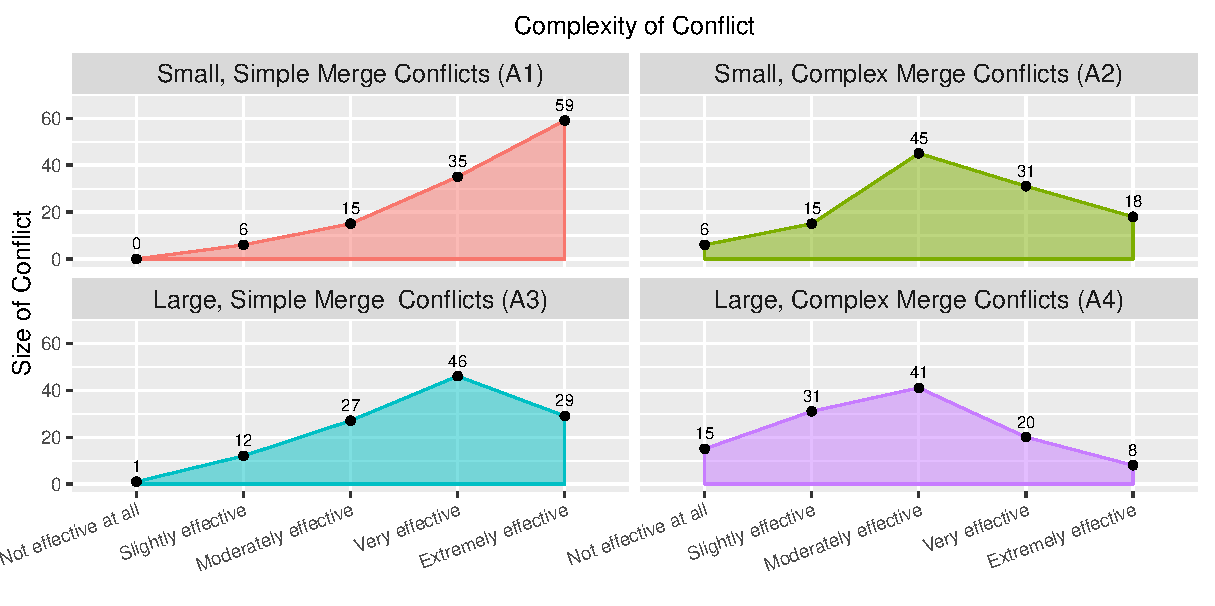
\includegraphics[width=0.92\textwidth]{ConflictComplexityVsSize.pdf}
%\caption{Effectiveness of practitioners' toolsets in supporting perceived size and complexity of merge conflicts, split on development experience. Bubble values indicate number of survey responses for effectiveness of a particular merge conflict size and complexity, and bubble size indicates the number of responses for comparison purposes.\vspace*{-0.5\baselineskip}}
%\label{size_vs_complexity}
%\end{figure*}

%\begin{table}[!htbp]
%\renewcommand{\arraystretch}{1.3}
%\caption{Practitioners' Trust in their Merging, History Exploration, and Conflict Resolution Tools\textsuperscript{i}}
%\label{survey_tool_trust}
%\centering
%\begin{tabularx}{0.65\textwidth}{@{}r|*{10}{C}c@{}}
%\toprule
%Trust Level & Response Count & Response \%\\
%\midrule
%Completely & 20 & 16.52\\
%A lot & 50 & 41.32\\
%A moderate amount & 41 & 33.88\\
%A little & 10 & 8.26\\
%Not at all & 0 & 0.00\\
%\bottomrule
%	\multicolumn{3}{c}{\noindent\parbox[t]{7.8cm}{\vspace{-3px}\textsuperscript{i}\hspace{0.2em}Survey respondents answered on a 5-point Likert-type scale indicating trust in their toolset (1 being \textit{Not at all} and 5 being \textit{Completely}).}}
%\end{tabularx}
%\end{table}

\subsubsection{Tool Mistrust/Transparency}\label{tool_trust}
Most merge tools attempt to resolve conflicts using a variety of algorithms, but revert to manual resolution when these algorithms fail.
Several interview participants indicated that they mistrust merge tools when they obscure the steps and rationale for particular results when resolving merge conflicts.
The opaque nature of history exploration tools was also found to be a source of practitioners' overall mistrust of their toolsets.
P4 commented:
\begin{quoting}
\textit{``I've never trusted the merge tools or diff tools... Sometimes I'll even manually go and do the merge myself rather than use a tool. Just because I've had several times where it's a bad merge, and I broke some code.''}
\end{quoting}

Based upon this theme of mistrust, we asked survey participants to rate the degree to which they trust their merging, history exploration, and conflict resolution tools.
We received 121 responses to this question, with a mean score of 3.66 placing the most common responses between \textit{a moderate amount} and \textit{a lot} of trust (Table~\ref{survey_tool_trust}).
Assuming that responses of \textit{a moderate amount}, \textit{a little}, or \textit{not at all} indicate some degree of mistrust, we find that 42.15\% of practitioners experience some gap in toolset trust.

However, the severity of toolset mistrust is not as significant as our interview results suggested.
Only 8.26\% of practitioners indicated that they trust their toolset \textit{a little} or \textit{not at all} (10 out of 121 responses).
As the results of the survey were counter to our interview results, we looked further. We found that: (1) participants reported on the trust levels of the tools that they regularly use, and (2) a large number of participants reported that they had discontinued toolsets when they ran into errors. This indicates that if participants had reported their trust level of these discontinued tools the results would have been lower.

\subsubsection{Perceptions of Tool Effectiveness}\label{tool_effectiveness}
The perceived size and complexity of merge conflicts affect the way in which practitioners plan, allocate, and enact resolutions.
To understand the degree to which these two factors impact practitioners' perceptions about the effectiveness of their toolsets, we asked survey participants to rate their toolset across four different merge conflict archetypes: (A1) \textit{simple, small merge conflicts}, (A2) \textit{simple, large merge conflicts}, (A3) \textit{complex, small merge conflicts}, and (A4) \textit{complex, large merge conflicts}.

Since individual participants have different toolsets, and consider different factors when determining the perceived size and complexity of a merge conflict, we instructed participants to rate their own toolset against these archetypes using their notion of what constitutes a simple vs. complex and small vs. large merge conflict.

Fig.~\ref{size_vs_complexity} provides a visual illustration of the results of this survey question.
The four plots display the results for each of the archetypes, with archetype (A1) in the top-left plot, (A2) in bottom-left plot, (A3) in the top-right plot, and (A4) in the bottom-right plot.
Individual plots are composed of a horizontal axis containing participants' software development experience, which we collect since experience can determine the range of conflicts that they have faced and their perceptions.
The vertical axis shows the range of possible responses for the effectiveness of merge toolsets.
The size and number within each bubble represent the number of respondents with a particular amount of software development experience that rated their toolset at that specific effectiveness level.

For example, a practitioner with 6-10 years of experience who indicates that her merge toolset is \textit{Extremely Effective} for \textit{small, simple merge conflicts} would be represented in the largest bubble (containing 19) in A1. % in the top-left plot. 
She would also be represented in the largest bubble (containing 13) in the bottom-right plot (A4) if she indicated that her merge toolset was \textit{Moderately effective} for \textit{large, complex merge conflicts}.

Observing the overall trends when moving between plots, we find that practitioners perceive complexity of the conflict to have a greater impact on the effectiveness of their merge toolsets than the size of merge conflicts.
Numerical analysis confirms this when finding that the mean response for archetype (A1) is 4.278 (where 5 is \textit{Extremely Effective} and 1 is \textit{Not effective at all}), (A2) is 3.782, (A3) is 3.347, and (A4) is 2.783.
The shift from \textit{small} to \textit{large} merge conflict size (A1 to A2) results in a difference in mean responses of 0.496, whereas the shift from \textit{simple} to \textit{complex} merge conflict complexity results in a difference in mean responses of 0.930.

These results suggest that merge tools are currently equipped to handle increases in the size of merge conflicts, but not as well equipped for increases in complexity.
The increasing amount of code being developed in distributed environments means that scaling support in both dimensions is necessary to accommodate practitioners' needs.